%!TEX root = thesis.tex

\chapter{Einleitung}

% Die Einleitung führt zum eigentlichen Thema dieser Arbeit hin. Dabei wird ein großer Bogen
% gespannt, in dem die Relevanz und der Kontext der untersuchten Thematik deutlich wird.
% Grundlegende Begriffe aus dem Titel und der Kurzfassung sollten aufgegriffen und definiert werden.
% Unterstützend können Zitate herangezogen werden, die der Arbeit einen Rahmen geben.

\section{Ziel der Arbeit}
Das Ziel dieser Arbeit ist es ein System zu entwickeln, welches den Reservierungs- und
Entleihprozess einheitlicher, effizienter und zufriedenstellender lösen lässt. Die Anwendung soll es
unter anderem ermöglichen, die auszuleihenden Assets in einer Liste abzubilden und diese zu
durchsuchen. Hierbei ist auch das Anzeigen einer Stückzahl der jeweils verfügbaren Assets, deren
Bedienungsanleitung sowie der verantwortliche Mitarbeitende sinnvoll.

\section{Forschungsfragen}
Es sollen die folgenden Forschungsfragen beantwortet werden:

\begin{enumerate}
  \item[\sffamily\color{maincolor} {F1}] {Welche zentralen Schwierigkeiten bringt die aktuelle Planung und Reservierung von Assets für Mitarbeitende und Studierende mit sich?}
  \item[\sffamily\color{maincolor} {F2}] {Was sind Anforderungen an ein System, welches die in F1 gezeigten Schwierigkeiten adressiert und reduziert?}
  \item[\sffamily\color{maincolor} {F3}] {Inwieweit kann ein aus F2 resultierender Prototyp die in F1 identifizierten Schwierigkeit reduzieren oder komplett minimieren?}
\end{enumerate}


\section{Vorgehensweise}
Die Entwicklung des Systems orientiert sich am menschenzentrierten Gestaltungsprozess
\cite{din_en_iso_9421-2102020-03_din_nodate}. Der Prozess teilt sich im Rahmen dieser Arbeit in
fünf aufeinanderfolgende Phasen (Abbildung 1), wobei die Entwurfs- und Implementierungsphasen
Spielraum für ein iteratives Vorgehen lassen. Unter anderem werden in der Analyse die Aufgaben des
Systems, die Benutzenden und der Kontext nach dem Entwicklungsprozess für interaktive Medien
\cite{herczeg_einfuhrung_2009} aufgeführt, um ein gebrauchstaugliches Ergebnis erzielen zu können.

\begin{description}
  \item[\ref{chapter-basics}] beschreibt die für diese Arbeit benötigten Grundlagen. In diesem
  Kapitel werden \ldots, \ldots und \ldots eingeführt, da diese für die folgenden Kapitel dringend
  benötigt werden.
  \item[\ref{chapter-konzept}] stellt das eigentliche Konzept vor. Dabei handelt es sich um ein
  Konzept zur Verbesserung der Welt. Das Kapitel gliedert sich daher in einen globalen und einen
  lokalen Ansatz, wie die Welt zum Besseren beeinflusst werden kann.
  \item[\ref{chapter-evaluation}] beinhaltet eine Evaluation des Konzeptes aus dem vorherigen
  Kapitel. Anhand von Simulationen wird in diesem Kapitel untersucht, wie die Welt durch konkrete
  Maßnahmen deutlich verbessert werden kann.
\end{description}

\begin{figure}[h]
  \centering
  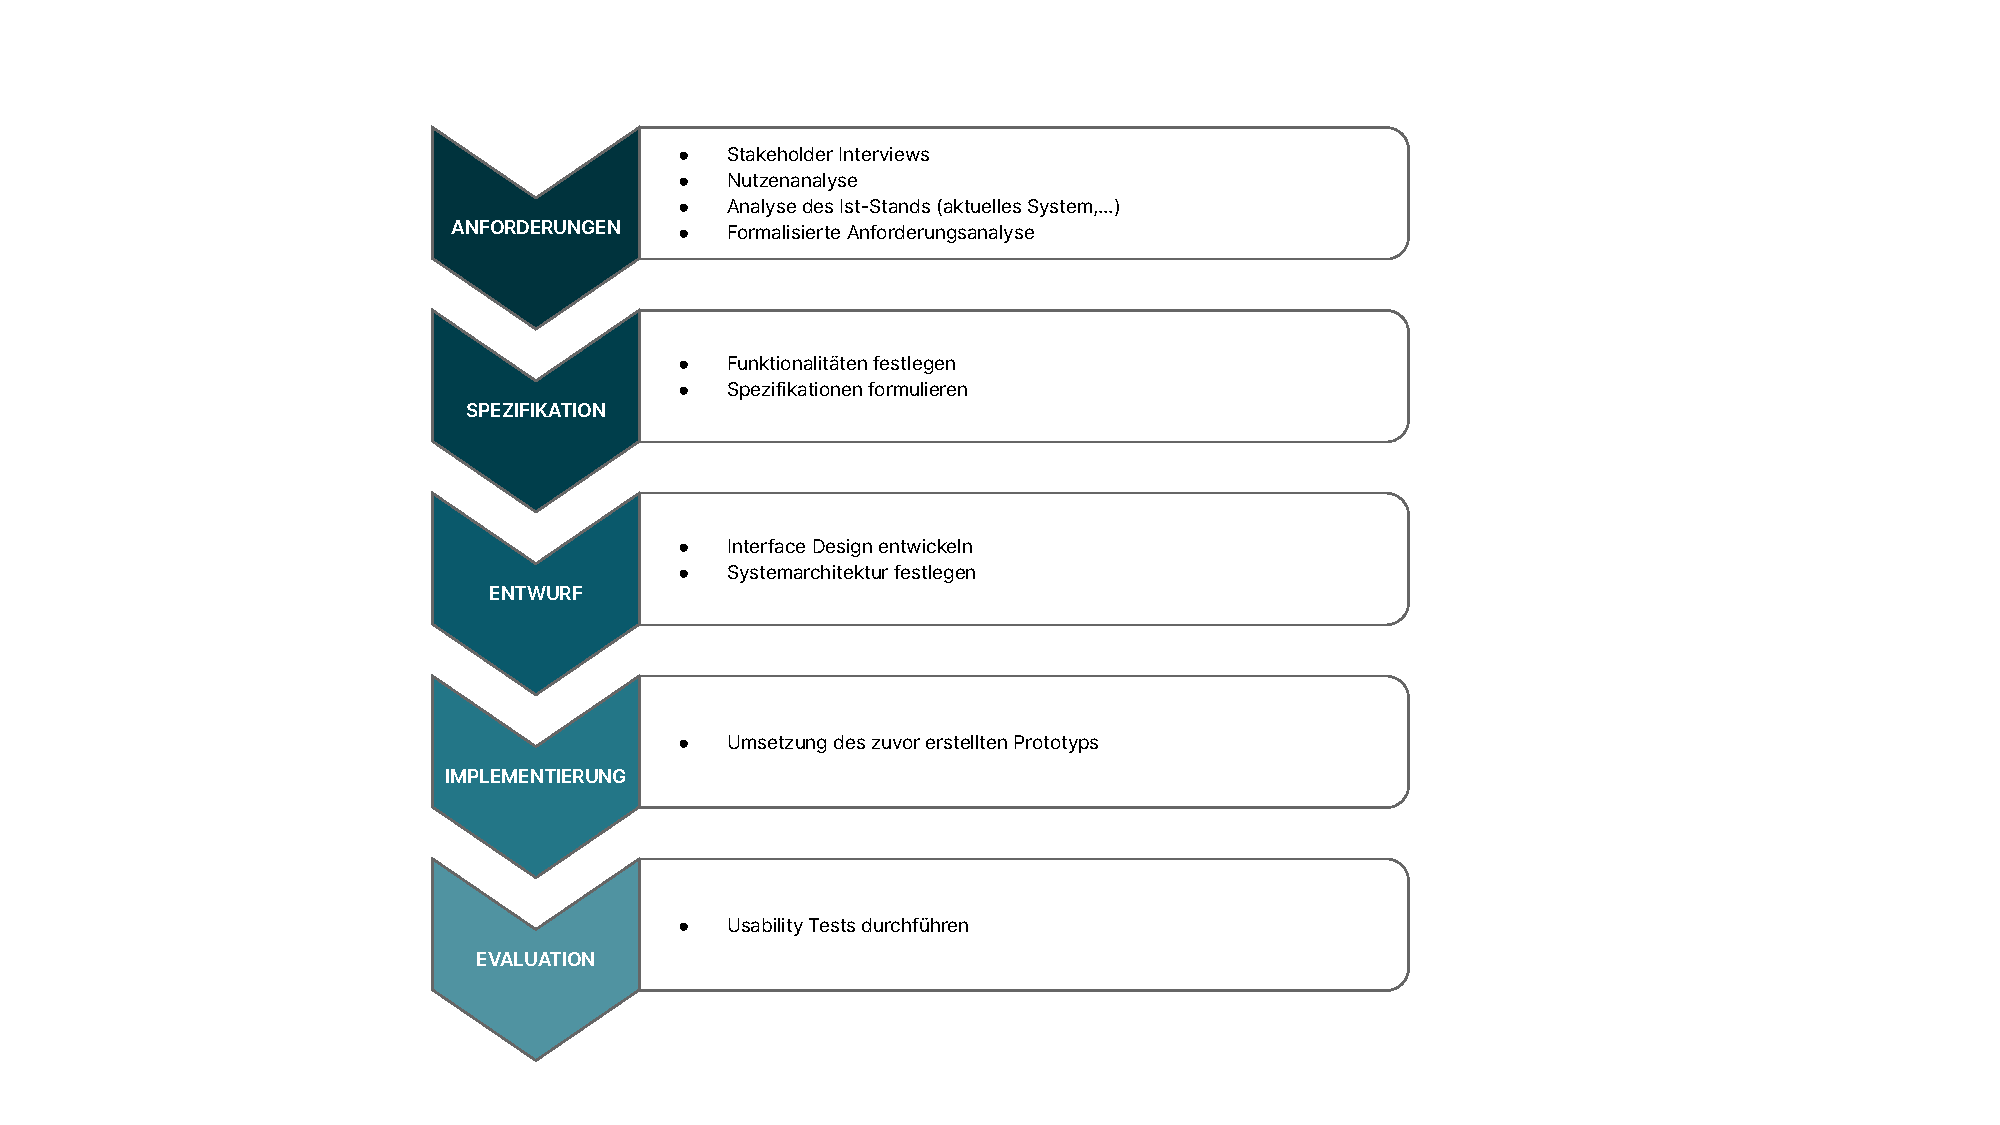
\includegraphics[scale=0.6]{Bilder/Vorgehensmodell.pptx.pdf}
  \label{fig:schablone}
  \caption[Vorgehensmodell]{Vorgehensmodell}
\end{figure}